\chapter{INTRODUCTION}
\label{chap:intro}

%intro here in one paragraph

The advent of big data sets has put pressure on the Mathematics and Statistics community to rethink how to apply traditional of analysis and inferencing. Both climate and oceanographic science disciplines are feeling this data explosion and are struggling to scale. Unprecedented amounts of data are made available by governmental agencies like \gls{noaa} and \gls{nasa}, and heavily used by the scientific community to draw inferences. The traditional visualization and delivery tools can be improved to handle a surge of new data delivery. The techniques used to visualize and retrieve these data needs to be reevaluated. Global predictions need modern web app technologies for professional and amateur to visualize and receive data quickly, accurately, and as painlessly as possible.

Traditional methods of parsing through a remote/local archive of files, selecting relevant files, opening the files and performing analysis on a single pc do not scale with big data. Scientists are spending more time navigating through data rather than finding discoveries. Worse still, amateurs in the form of young people, hobbyists, students and potential scientists get frustrated and give up on using these rich data sets. Toolkits and web apps are suggested in this thesis to relieve this pressure. Modern \gls{restfull} app design gives the community a walking stick to help them wade through the big data mire.

It's worth mentioning here another big data paradigm. Distributed systems/cloud computing offers the scientific community a means to handle big data at the expense of complicated overhead and expensive cloud-based services, such as \gls{aws}. Most scientists do not want, or in many cases do not even need these services. They need a subset of big data, or to be able to break down a data set into smaller pieces for their studies. Cloud computing services do not address the issue of accessibility and visualization. Comparing toolkits/web apps to cloud platforms are not opposing viewpoints. Instead, they can be used (or not) to varying degrees.

An unsettling reality is that as new technologies unfurl, mathematicians, statisticians, and scientists are pressured to adopt them without question or complaint. Expecting the community to embrace new paradigms is impracticable, and branding scientists who are reluctant to embrace as 'old school' manifest the fallacy that new is better, young outpaces the old, and what you learned yesterday has no use today. This fallacy also cloaks the issue with these new paradigms: they are not needed for most scientific applications. In the context of the problem posed in this thesis, we are interested in big data visualization and delivery, and tailor this solution to what the community wants/needs. In this scope, big data is divided piecemeal into relevant sections that can be visualized and delivered with minimal domain expertise.

Time series analysis and gridded interpolation of climate systems are usually done on local spatiotemporal realms. The mathematical models that describe complex systems simplify climate regimes to seasonal, spatial, and temporal scales small enough to be computed on a single machine. A butterfly's flapping its wings in the Amazon is not modeled for Gulf rainfall after all! In this sense, the methods used to simplify the data is under investigation. Models are evaluated by how well they fit different data sets, and it is of interest to the community to try as many models as possible and to compare results with each other. In this sense, data visualization and accessibility aid the scientific process, as it allows ease of data for modeling, and is means of comparing. In the next sections, we hope to introduce current visualization platforms available for two different datasets. A 3D gridded satellite product, and a 4D in situ ocean sensor array product.

\section{Background and significance of visualizing spatial data using smart phones}

The daily snow and ice coverage dataset over the Northern Hemisphere (NH)
based on the Interactive Multisensor Snow and Ice Mapping System (IMS) maintained by the United States' NSIDC \cite{NIC} is a useful tool for numerous applications, such as monitoring day-to-day weather variations for water resources and agriculture, and estimating the snowstorm severity for insurance industries and governmental agencies. 
The IMS data derives from remote sensing of multiple satellites, including NOAA POLES satellites,
MODIS Aqua and Terra, as well as {\it in situ} observations. \cite{fetterer2011ims,ramsay1998interactive}
The dataset began on 4 February 1997 and has numerous users, ranging from professionals including climate scientists, satellite remote sensing experts, hydrological engineers to high school students and climate science enthusiasts. A few visualization sites cater to this broad audience, offering a quick visualization platform. 

Rutgers University Global Snow Lab provides a daily snow-cover \url{https://climate.rutgers.edu/snowcover/} \cite{rutgers_sl}. Here users can scroll through preprocessed images of the daily snow cover. Visualization is limited to scrolling through images. There are no zooming features, or time series offered.

The United States National Snow and Ice data center provide another image archive at \url{http://www.natice.noaa.gov/ims/} \cite{nat_ice}. Here users also can download images of IMS’s daily northern hemisphere snow and ice coverage. Additionally, they can view and download United States, Alaska, Europe/Asia, and Afghanistan regions. As with Rutgers site, the users are unable to zoom or download the actual data. Furthermore, the actual square coverage for this site is limited to pixels on an image. Estimating square km areas are limited to a 3-day mean ice coverage chart, showing maximum and minimum bars along with a dotted line average shown in Figure~\ref{fig:nat_ice}

\begin{figure}[ht]
  \centering
  \begin{minipage}{4.5in}
    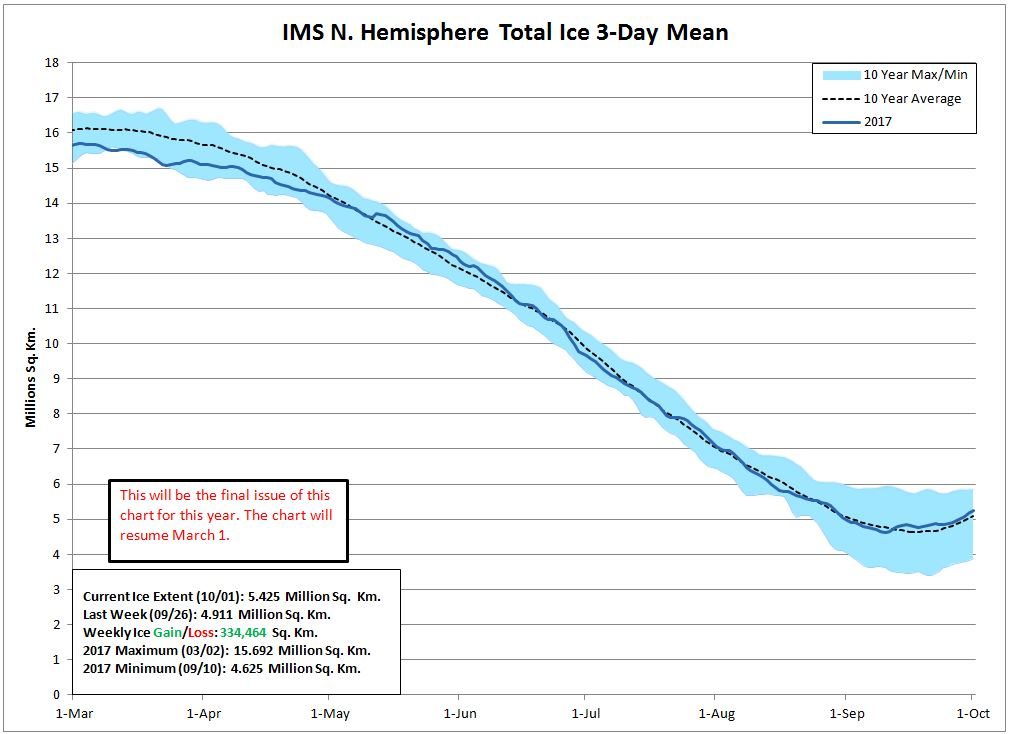
\includegraphics[width=\linewidth]{ims_data.jpg}
    \caption{ \label{fig:nat_ice} Sea and Lake Ice coverage of IMS data using 4 KM resolution. Ice coverages are calculated using a three day running mean from March until September each year. Blue border displays maximum and minimum values for the season. Areas are calculated using the Lambert Azimuthal Equal Area Projection with a WGS84 Datum. \cite{nat_ice}}
  \end{minipage}
\end{figure}

Users are left to examine two figures with square kilometers provided but are not able to see how the area is calculated. The IMS' calculation of the actual snow-covered area based on each grid box needs clarification. Because IMS provides images on a polar stereographic projection, the pixel area is a distortion of the true square kilometer coverage. Projecting a three-dimensional sphere/ellipsoid on a 2d plane using a stereographic projection stretches out low latitude areas and contracts high latitudes \cite{snyder1987map}. The IMS community would benefit to know how to make this calculation, or better still, have software calculates the true area for them.

Chapter 2 of this thesis describes a software toolkit written in Python that calculates areas of the coverage provided by the Northern hemisphere. This toolkit also parses through the IMS data set for a given latitude-longitude. This thesis shall provide the theoretical basis for the toolkit, along with a time series analysis of the Tibetan Plateau Area. This toolkit is used by the Institute of Tibetan Plateau Research Chinese Academy of Sciences to produce daily snow coverage images located at \url{http://www.tpedatabase.cn/tibetSnow.jsp} \cite{TP_database}. 

Information and improvements regarding the toolkit shall be discussed, chiefly the opportunity for the creation of a web application that provides users with visualization and data retrieval built with modern website technology. Providing the source code limits the users to those who know Python; on the other hand, a web app connected to an intuitively designed user interface is a pragmatic way to serve the current IMS community to expand its user base.


\subsection{Past work}
\subsection{Current scenario}
\subsection{Future work for quick visualization and analysis of big data}



\section{Motivation of the VACYD research: crop yield data visualization}

For over a decade, the Argo program has provided temperature, salinity and pressure data (T/S/P) on a global scale for depths as far as 2000 decibar (dbar), with unprecedented spatial and temporal resolution and no seasonal bias \cite{argo}. Close to two million profiles have been collected and made publicly available on Argo’s Global Data Assembly Centres (GDACs) on \gls{ftp} servers. Data is recorded by various types of floats that drift at a resting depth and raise every few days to transmit information to GDACS. From there data underwent quality control markers and adjustments and released as a \gls{NetCDF} product on FTP servers. Users can download either profile (one cycle of a floating measurement) or the entire profile history of a float. Though there are visualization tools available, almost all of them do not allow querying based on a spatial-temporal selection. For example, retrieving Argo profile data for North Sea regions at a certain depth and date. Chapter 3 will describe a web app that is used to allow such a data retrieval service.

\section{A short summary of the app development method and results}

Argo floats are equipped with an inflatable bladder, allowing them to float and sink. Once deployed the floats are programmed to drift at a 1000 meter depth for nine days. After nine days before descending to 2000 meters, then rising at a rate of 10 cm/s. While ascending the float sensors begin sampling parameters described in Table~\ref{tbl:argoParams}. Ascension takes 6 hours. Once at the surface the float transmits data via satellite to the GDAC, taking 6-12 hours for floats using the Argos1 and Argos2 satellite systems. \cite{argo_uk}.

As early as 2005, floats with GPS navigation have been introduced \cite{argo_man}. Iridium and Argos-3 satellite systems data transmitted in a matter of minutes. The ratio of ARGOS to GPS floats is displayed over time by Figure ~\ref{fig:commTS}, collected from the Argovis database. According to this plot, Argos makes up $\approx 36\%$ of all profiles released, and GPS makes up $\approx 64\%$. Not only is GPS faster, but also allows higher frequency sampling. Floats that use GPS transmit $\approx 1000$ samples for each parameter. In contrast, Argos1 and Argos2 transmits only $\approx 100$. The Argo dataset is growing as more floats are deployed \textit{and} with increased sampling rates.

\begin{figure}[ht]
  \centering
  \begin{minipage}{4.5in}
    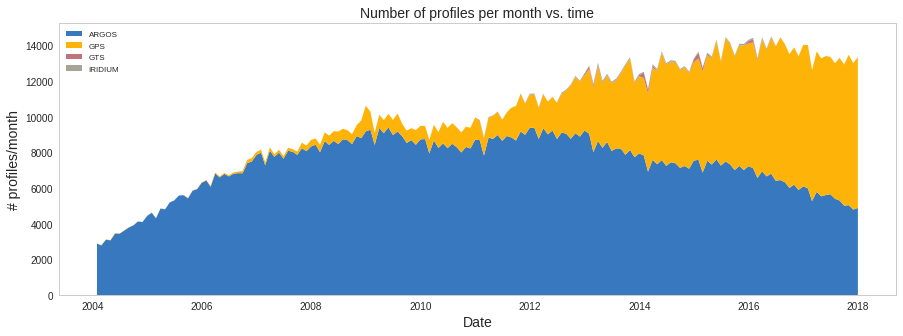
\includegraphics[width=\linewidth]{commTS.png}
    \caption{ \label{fig:commTS} Satalite Communication Type by month. Iridium floats also use the GPS system.}
  \end{minipage}
\end{figure}

\begin{figure}[ht]
  \centering
  \begin{minipage}{4.5in}
    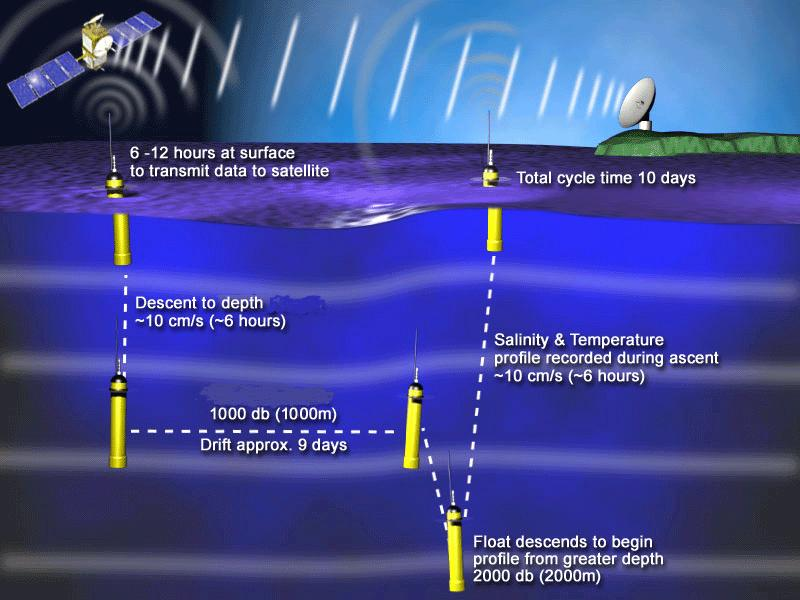
\includegraphics[width=\linewidth]{operation_park_profile.jpg}
    \caption{ \label{fig:argo_cycle} Detail of one profile cycle\cite{argo}}
  \end{minipage}
\end{figure}

\section{Literature review}